\chapter{Background}


In this chapter will introduce all the background that is helpful to understand the rest of the Thesis. 
First off, it will explain what the USB protocol is and how it works, next the kind of attack this thesis deals with, and finally the hardware that is involved, specifically the O.MG cable. 

\section{The USB Protocol} \label{TheUSBProtocol}

The USB standard was first published in 1996 [SOURCE MISSING]. It was developed in a collaboration between the tech companies Compaq, DEC, IBM, Intel, Microsoft, NEC, and Nortel as a new standard to connect slow peripheral devices. To this end, they founded a new non-profit, called the USB Implementation Forum \cite{USBIFUSBIF}. It's goal were:
\begin{itemize}
    \item "Ease of use for PC peripheral expansion"
    \item "Low-cost solution that supports transfer rates up to 12 Mbs"
    \item "Full support for the real-time data for voice, audio, and compressed video"
    \item "Protocol flexibility for mixed-mode isochronous data transfers and asynchronous messaging"
    \item "Integration in commodity device technology"
    \item "Comprehend various PC configurations and form factors"
    \item "Provide a standard interface capable of quick diffusion into product"
    \item "Enable new classes of devices that augment the PC's capability"  
\end{itemize}
It is apparent, that the creators wanted an universally applicable standard protocol, for all sorts of data connections, that is also flexible, and on top of all that easy to use and low in cost. Their solution was the Universal Serial Bus.

\begin{figure}
    \centering
    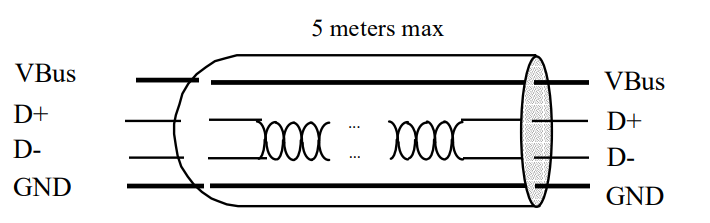
\includegraphics[width=0.5\linewidth]{usbsingalgraphic.png}
    \caption{USB Cable Signals}
    \label{fig:usbsingalgraphic}
\end{figure}

Connection is built upon four signal lines; a negative (Ground) powerline GND, a positive powerline VBUS for the power supply, and two data transfer lines D+ and D- as depicted in \ref{fig:usbsingalgraphic}. The two physical transfer data lines are aligned as a twisted pair. This alignment protects them from outside noise but does not mean that more than one logical line is available. They work together to transmit just logical signal, one bit. USB utilizes Non Return to Zero Inverted (NRZI) meaning that the bits on the bus are represented by a transition of physical levels, rather than the presence or absence of them. This allows data transfer while simultaneously allowing the participating parties to synchronise their bit clocks.  \\
Since there is only one logical data line, data transfer can only happen in one direction at a time. Bi-directional communication happens in half-duplex mode. To deal with this restriction, a protocol that manages data and sender order has to be followed; the USB protocol.  

This next section will expand on the functionalities of the USB protocol as described by \cite{nissimUSBbasedAttacks2017}. 

A USB connection includes a host, usually a computer, and one to many peripheral devices that connect to the PC's embedded USB hub.  \\
USB devices generally fit into two categories; I/O devices that add capabilities to the host, and hub devices which connect additional devices to the host. An USB cable has two main functionalities; Establishing a data connection allowing communication between the connected parties, and supplying electrical power to the connected peripheral device if it is not self-powered. Such devices that draw power from an USB Host are called bus-powered. \\ 
For bus-powered devices it is important to receive the power from the UBS cable before it is supposed to process any data, which is why the USB connector was specifically designed with power pins that are longer than the signal pins.\\
Every USB device is equipped with a microcontroller chip that manages the USB interactions with the host, and optionally also has a bootloader that allows loading firmware, for example for updates. \\
One USB device consists of one to multiple logical subdevices that are known as device functions. For a webcam with built in audio this would correspond to a video and an audio function. Devices with multiple subdevices are referred to as composite devices. Each functions is managed through a separate endpoint on the bus with it's own logical address. One endpoint forms a logical communication channel called a pipe, of which there are two types.  
\begin{enumerate}
    \item Message Pipe: A message pipe is used for control transfers. That means they re used for short and simple commands sent to the USB device and status responses to the host.
    \item Stream Pipe: A stream pip is used for actual data transfer.
\end{enumerate}
Data transfer can only take place, if the host directly requests it. An USB device cannot transfer information autonomously. 

In order to be able to communicate with any USB device, a connection needs to be established and initialized. This is done with a process called 'enumeration' that starts as soon as the physical connection is established. It consists of four main steps;

\begin{enumerate}
    \item \emph{Detection}: A change in the current on the data lines is detected by the host, so it knows that a new USB device has been connected.
    \item \emph{Device Speed}: The speed of the device is determined by using the change on  the data lines in step 1.
    \item \emph{Device Descriptors}: The USB device is reset by the host through a specific dataline signal. This prompts the device to send information about itself (it's descriptors) to the host by which it is identified.  \\
    The exchange of descriptors follows a defined order; 
    \begin{itemize}
        \item First the host will request the descriptor length and the descriptor from the device with the Get\_Device\_Descriptor command.
        \item The advice is reset again and given a unique local address by the host called via the Set\_Address command. 
        \item Lastly, the device is prompted to send it's configuration by the Get\_Configuration\_Descriptor. The configuration includes a hierarchy of interface, endpoint and class specific descriptors.  
    \end{itemize}
    \item \emph{Loading Drivers}: Now that all the information has been exchanged the host can start using it to load the device specific driver's that will allow it to be controlled. The corresponding driver is found by the USB class, the vendor ID (VID) and the product ID (PID). Most standard drivers are included in the OS of the host, if they aren't the user has to download them manually. This concludes the enumeration process, after these steps the device is ready for use.
\end{enumerate}




\section{The Dangers of USB}

Some people might notice that during the initialization process described in section \ref{TheUSBProtocol} there is not verification or authorization steps. The protocol assumes that and physically connected USB device is trustworthy and does not take any precautions to check it's claims and properties. \\
This is a big oversight and opens the door for a lot of malicious activity. 
On top of that USB devices are not perceived as a threat by a vast majority of people. In fact, many would absolutely pick up, plug in, and even interact with USB sticks they find lying around on the ground \cite{tischerUsersReallyPlug2016}. A study \cite{tischerUsersReallyPlug2016} conducted in 2016 found that USB sticks are a very effective attack vector. They explored whether USB sticks dropped on a university campus would really be picked up and plugged in. They found that users opened one or more files on 45\% of the flash drive and that 98\% of the drives were removed from the drop location by the time the experiment had ended. Based on this, the authors estimate that between 45\% and 98\% of drives were eventually plugged in. On the drives the authors placed information for a survey to explore the finder's motivation. From this survey it was concluded that the USB drives were plugged in mostly out of altruistic motives (to find the owner). The social engineering attack was an "expeditious" vector with a median time of connection of only 6.9 hours.  \\
USB ports are common also in public, for convenient charging on the go, for example in Buses or Airports \cite{kumarJuiceJackingUSB2020}. People rarely think twice when they connect their laptop to an external display in a library or accept a charging cable from a friend. But for none of these actions are there any security measures in place, a newly connected USB device does not have to provide authentication.

A myriad of different attacks are possible through such an unsecured attack vector, \cite{phamUniversalSerialBus2011} divides them in an online and an offline attack mode. \\
\emph{Offline Attack Mode:} Since 2005, when USB 2.0 was released and found it's way into corporate environments, data theft became a big concern. Through USB, data can be silently downloaded without the user's permission or knowledge from computers \cite{clarkHardwareTrojanHorse2009} as well as phones \cite{SharpIdeasDownloads2006}. USB drives developed to be able to do data manipulation, and with the increased popularity of U3, attackers could hack U3 images and replace them for their own malicious purposes to take advantage of auto-run. 
How much damage could be done with this is best exemplified with Stuxnet \cite{kushnerRealStoryStuxnet2013}. It's a malware program that could travel via USB; a computer that came in contact with an infected USB stick would immediately be compromised. In this way, malware could spread even in an air-gaped environment. The highly sophisticated and targeted attack was discovered in 2010 and is confirmed to have damaged centrifuges that were part of Iran's Nuclear Program.\\
But an attack via USB does not have to have the dimensions of an (alleged) geopolitical intelligence mission \cite{kushnerRealStoryStuxnet2013}, there are more examples of day-to-day threats to exemplify what USB can do. On Windows XP it is possible to emulate a CD-ROM device through an USB connection and hack the U3 autoplay feature \cite{al-zarouniRealityRisksConsented2006}, data can be exfiltrate from iOS6 through a USB charging cable \cite{lauMactansInjectingMalware2013}, USB can be used to propagate attacks from one computer to another, as demonstrated in \cite{wangExploitingSmartphoneUSB2010}, or destroy a target with power surges that irreparably damage the host \cite{USBKillDevices}, and, most importantly, since USB does not require authentication, it can be used to emulate other devices, namely devices that are used for human input. Human Interface Devices (HID) such as keyboard and mouse present an unparalleled attack vector, where a hacker with physical access to an unlocked computer can remotely do any action a user themselves could do \cite{USBRubberDucky}, \cite{MGCable2019a}, \cite{lawalFacilitatingCyberenabledFraud2022}. \\
How such HID attacks could look like, and what 